\documentclass[12pt,onecolumn]{IEEEtran}

\usepackage{rotating}
\usepackage{tikz}
\usepackage{booktabs}
\usepackage{multicol}
\usepackage{tabularx}
%\usepackage{color}
\usepackage{xcolor}
\usepackage{lastpage}
\usepackage{fancyhdr}
\usepackage{grffile} 
\usepackage{graphicx}
\graphicspath{ {images/} }
\usetikzlibrary{arrows, positioning}
\usepackage{amsmath}
\usepackage{newfloat}
\usepackage{caption}
\usepackage{mathtools,cuted}
\usepackage{lipsum}
\usepackage[final]{pdfpages}
\usepackage{lettrine}
\usepackage{siunitx}
\usepackage{pgfplots}
\usepackage[europeanresistors]{circuitikz}
\usepackage{listings}
\usepackage{verbatim}
\usetikzlibrary{arrows}

\lstset{frame=tb,
language=matlab, 
breaklines=true, 
showstringspaces=false, 
columns=flexible, 
numbers=none,
commentstyle=\color{green},
tabsize=3
}

\pgfplotsset{compat=1.14}

\begin{document}
\author{Marion Heimann - 788579 \\ Tristan Kuisis - 812587}
\title{ELEN4002 - Lab Project Plan \\ Preliminary Report on the Design and Creation of a Wits Analytics and Visualization of Energy Systems}
\maketitle
\begin{abstract}
    The main purpose of this document is to outline a project plan for the data analytics and visualization of energy systems across the multiple Wits campuses. The multiple energy meters installed across the properties have been gathering data for a number of years. A web server is constructed that is capable of autonomously and repeadly drawing the data from the database. The server will then host a portal that is capable of displaying the data to a user. The web portal will also be used to generate unique visualizations of the data from the sensors.
\end{abstract}
\begin{IEEEkeywords} 
Selenium, 
\end{IEEEkeywords}
\pagestyle{plain}



\section{Introduction} \label{sec:Introduction}
\IEEEPARstart{T}{his} report details the project plan for the data analytics and visualization of energy systems that make up the Wits campuses. 

There are a number of large energy requirements that Wits has-electricity, water, natural gas, petrol, diesel, as well as a number of other resources which make up smaller fractions of the universities energy usage.

This project, firstly makes use of the electricity meters installed throughout the buildings on the properties. These meters have been providing data for varying amounts of time, as well as data outages occurring occasionally (this will have to be dealt with). 
The wealth of information that these data loggers provide allow for the creation of a web server which is capable of drawing this data from the database, and making use of this data to visualize the energy usage across Wits. The web server will be instrumental in allowing a user to visualize this energy in a multitude of ways. 
The timelines, methods, tools, and a number of other details are discussed throughout this report.


\section{Project Specifications}

\subsection{The Data} \label{sec:TheData}
As discussed above, there are a number of energy meters placed throughout the Wits properties. There are approximately 310 data loggers that are connected to the current web portal used by the university. 
The system in place, run by IST \cite{IST}, is based off-campus. This means that their web service and data is housed on their side. All of the data retrieval (from the data loggers) is done through the Wits network and through in some cases through mobile data. This element of the project is discussed further down in sections \ref{sec:DataConversion,sec:DataGathering,sec:DataManipulation}. 

There are two other highly relevant data sets that will be used for the core part of the project. These are: the energy generated by the solar panels placed on top of a number of buildings throughout campus, and the weather of Wits. 
These two data sets will allow for a unique picture to be painted which further enhances the visualization of the system as a whole. 

Currently, this is the chosen data sets that will be used for the core of the project, however, if time permits, the university holds a wealth of information regarding the location of individuals throughout the university, this is provided with the use of the Integrated Campus Management (ICAM) system which is used for the access control for the university. 
This system is likely to unlock further insights on the universities energy usage and how the movement of individuals affects the energy usage of specific areas. 


\subsection{Back-End} \label{sec:BackEnd}
In order to run the system proposed, a number of operations are required to take place in a selection of programming languages, and all of these should be able to communicate with one another such that the process described by .... can take place. 

The back-end can be described by a local web server that is run on the users machine (in this case, the server is run on each ISTPassword' personal computer), and it is important as it allows the simulation of a server that will (ideally) eventually be placed onto a standalone system such that users with access to the internet will be able to use the system anywhere.
This section is discussed in further detail in section \ref{sec:server}.

\subsection{Front-End} \label{sec:FrontEnd}
In order to allow for the visualization of energy, the use of standard front-end web tools will be employed in order to provide the user with interaction. 
The back-end will provide all of the processing requirements, and will manage the data. the front-end communicates with the back-end (server) in order to illustrate the required information.
The three main tools (commonly used in any website), are: Hypertext Markup Language (HTML), Cascading Style Sheets (CSS), and JavaScript. 
These three tools communicate with eachother and the server in order to provide the user with the required information when viewed from a web browser. 

It is this part of the system where a multitude of visualization tools are used to gain insights into the data. These tools will be discussed in section \ref{sec:ApplicationsAndTools}

This completes the overall description of how the system is constructed and how it functions in order to get the required functionality.


\section{Scope Statement} \label{sec:ScopeStatement}
There are four sections to the scope for this project, these are: data gathering, back-end system, front-end system, and the ability to use the front-end system to gain insights. All of these sections for part of the scope for the project. 

The data gathering is required to be capable of autonomously and periodically draw data from the IST server for all of the 

Pick a focus: something to attain (see how money works or how new lights changed things)

Demonstrate concept


\section{Timeline} \label{sec:Timeline}
WBS?

\subsection{Working Times} \label{sec:WorkingTimes}
8-5
documentation


\subsection{Milestones and Deliverables} \label{sec:MilestonesAndDeliverables}
WBS?

Meetings with stakeholders + implement their suggestions


\section{Risks} \label{sec:Risks}

\section{System Architecture} \label{sec:SystemArchitecture}

\subsection{Website/Portal Architecture} \label{sec:WebsiteArchitecture}

\begin{enumerate}
\item Prepare for the activity of sitemapping
\item Brainstorm the types of content
\item Define primary navigation
\item Flesh out second and third level structure and content
\item Don’t forget about utility pages
\item Create notes and high-level specifications for each page
\item Designate the type of design template
\item Iterate. Iterate. Iterate.
\end{enumerate}

Maps which illustrate how one navigates through the website. 

\section{Resources} \label{sec:Resources}

\section{Applications and Tools} \label{sec:ApplicationsAndTools}

\section{Development Approach} \label{sec:Development Approach}

agile, waterfall, scrum

Testing methods

\section{Dependencies} \label{sec:Dependencies}


\section{Licensing} \label{sec:Licensing}

\section{Documentation} \label{sec:Documentation}

\section{Interfaces} \label{sec:Interfaces}

\section{Server} \label{Server}
\section{Data Gathering} \label{sec:DataGathering}
weather data

The system has a collection schedule set at thirty minutes, this means that each of the data loggers is sent a request, and the data is the sent to the IST servers, where it is stored in their database. 


IST host a web service which allows customers to view the relevant information from these data loggers. 
The web portal allows the user to view a range of details about the system, the homepage of the system is illustrated in Fig.~\ref{fig:ecwin}.

\begin{center}
    \begin{figure}[htb]
        \centering
        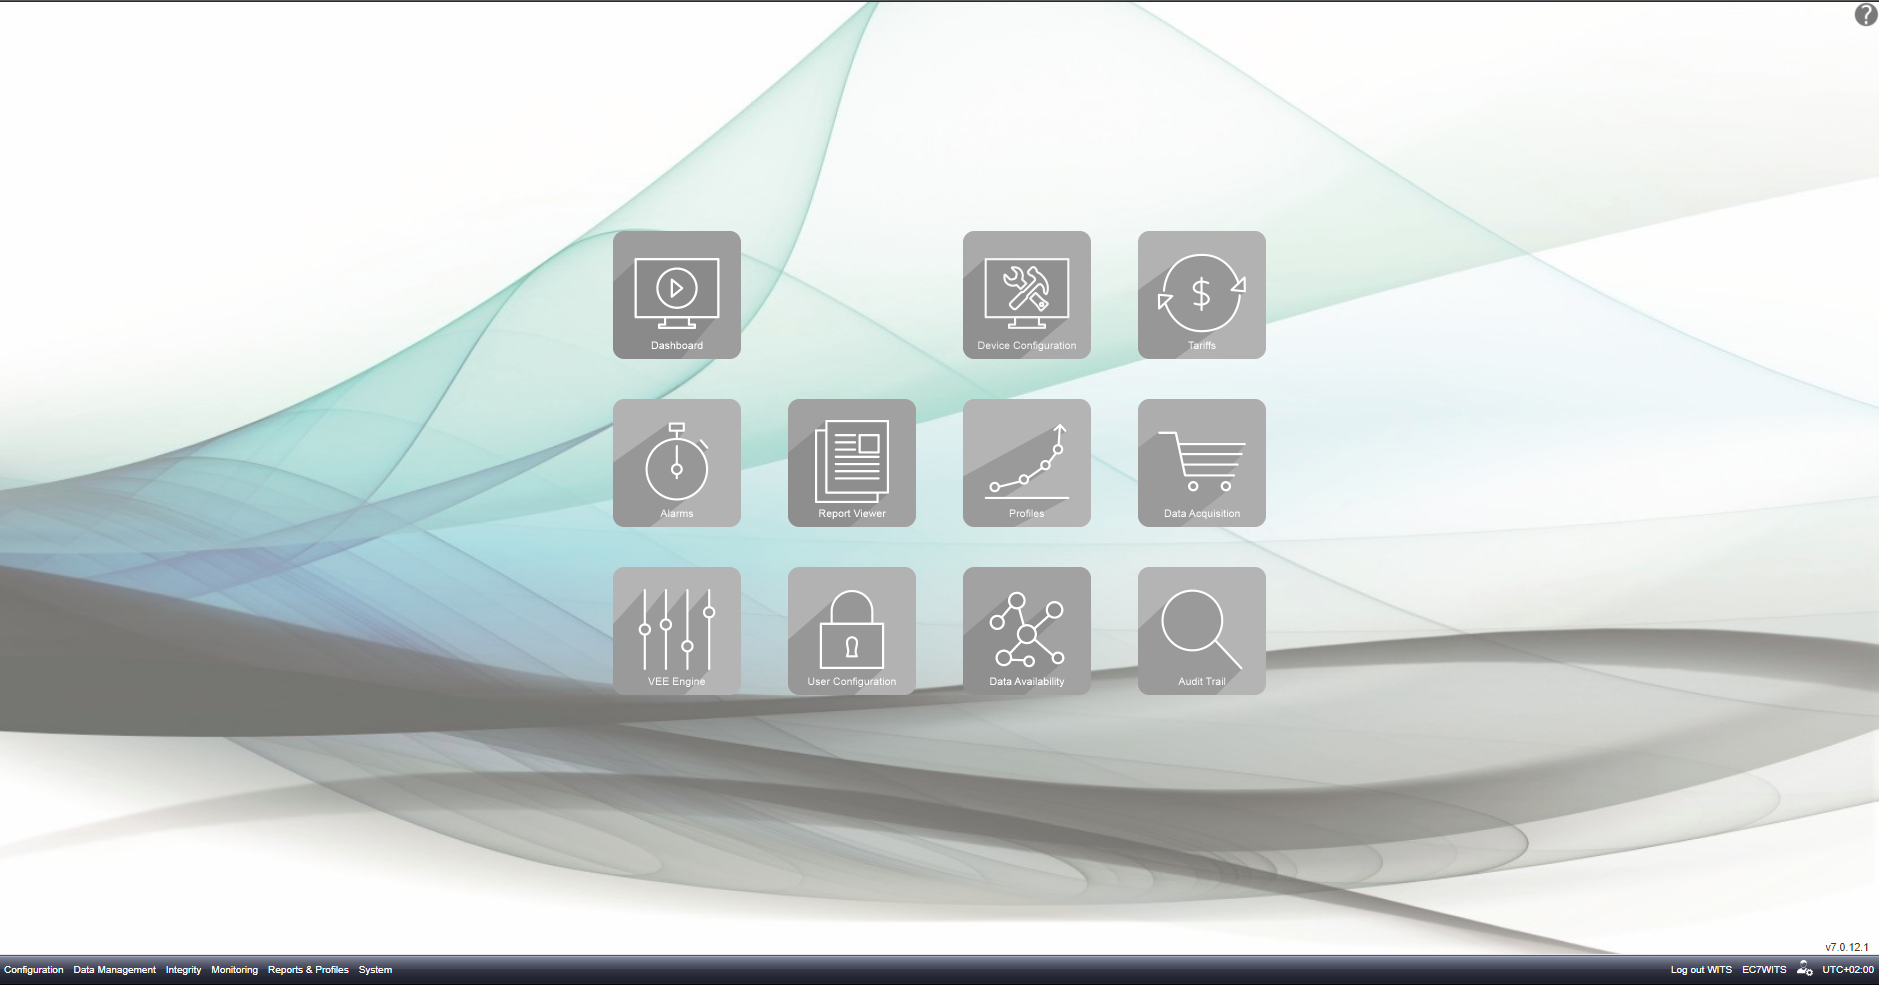
\includegraphics[width=0.8\textwidth]{ecwin.png}
        \caption{ecWIN Web Portal}
        \label{fig:ecwin}
    \end{figure}
\end{center}

This is the web portal that is to be used to gather the data from, this can be done by navigating to two different sections of the system: through the data editor section, and through the reports section. Both of these are, however, limited in their functionality. It must be noted that access to the IST database directly has not been granted as of writing this report, this is why the following methods have been utilised.

The data editor has a major shortfall in that one can only view the data loggers' data in small intervals, this means that when gathering the data for the specific meters, the system will have to download multiple files and then stitch them together to get complete representation of the data from that meter.

The reports section allows the user to view the data with no limits on the date range, however, when one selects the option to export the data, an error occurs (illustrated in Fig.~\ref{fig:error}). 

\begin{center}
    \begin{figure}[htb]
        \centering
        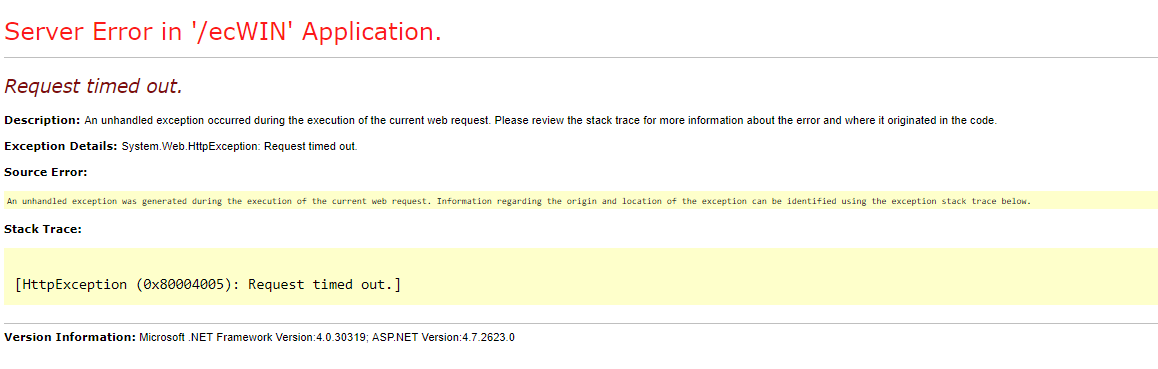
\includegraphics[width=0.8\textwidth]{ecwinerror.png}
        \caption{ecWIN Data Export Error}
        \label{fig:ecwinerror}
    \end{figure}
\end{center}

Thus, the choice of gathering the data from the data editor is chosen, and the method of gathering this data is further discussed in section~\ref{sec:sec:DataGathering}.

% Firstly to download all of the data going back... Then once this has happened, keep downloading the data periodically.
% A system must be in place so that the system can check up on the validity of the data that it has downloaded and compare it to the data on the server. 

\section{Data Conversion} \label{sec:DataConversion}

\section{Data Manipulation} \label{sec:DataManipulation}

\section{Accessibility} \label{sec:Accessibility}

\section{Insights} \label{sec:Insights}


\cite{datasite}

\bibliography{IEEEabrv,References}
\bibliographystyle{IEEEtran}
% \newpage
%\onecolumn
%\appendix


\end{document}